\documentclass{ctexart}
\usepackage[utf8]{inputenc}
\usepackage{amsmath}
\usepackage{hyperref}
\usepackage{cite}
\usepackage{tikz}  
\usepackage{graphicx}  
\usepackage{subcaption}

\usetikzlibrary{positioning}  

\title{用简单神经网络实现 MNIST 数据库手写数字识别的 C 语言实现}
\author{Andrew Carter \\ University of Warwick \and Kimi Ai \\ 月之暗面 
\and ChatMate \\ 浙江大学 
\and Crazyfish\footnote{wang\_heyu@msn.com} \\ CC98}
\date{}

\begin{document}

\maketitle

\section{导言}
\label{sec::introduction}

\subsection{MNIST 手写数字识别问题}

手写数字识别是计算机视觉领域的一个经典问题, 它的目标是开发出可以识别手写数字的算法或模型.
这个问题在实际应用中有广泛的应用, 例如邮政编码识别、银行支票处理和表单自动化处理等\cite{lecun1998gradient}.

MNIST (Modified National Institute of Standards and Technology database)
数据集是手写数字识别问题中最常用的一个基准数据集. 它由美国国家标准与技术研究院 (NIST) 的员工和美国的高中生手写的数字构成.
该数据集由美国国家标准与技术研究院在 20 世纪 80 年代收集, 然后由 Yann LeCun 等人进行修改和发布\cite{lecun2010mnist}.

MNIST 数据集的目标是作为一个简单的计算机视觉数据集, 用于训练和测试各种机器学习模型.

MNIST 数据集包含了 70000 个样本, 每个样本都是一个 $28 \times 28$ 像素的灰度图像,
代表了数字 0 到 9 之一. 这些样本被分为两个子集: $60000$ 个样本用于训练,
剩下的 $10000$ 个样本用于测试. 每个样本都有一个对应的标签,
表示图像中的实际数字\cite{simard2003best}.

在 MNIST 手写数字识别问题中, 我们的任务是根据输入的图像预测出对应的数字. 为了解决这个问题,
我们需要设计并训练一个机器学习模型, 例如神经网络, 使其能够从图像中提取出有用的特征,
并基于这些特征进行预测\cite{ciresan2012multi}.

这个问题的挑战在于手写数字的巨大变异性, 包括笔迹的粗细、数字的形状和大小、书写风格等.
此外, 由于图像的维度相对较高 ($28 \times 28 = 784$), 因此需要处理高维数据的复杂性.

总的来说, MNIST 手写数字识别问题是一个很好的入门级机器学习问题, 它需要处理实际的图像数据,
同时问题的规模和复杂性也适中. 通过解决这个问题, 我们可以学习和掌握许多机器学习的基本概念和技术.

\subsection{神经网络的基本概念}

神经网络是一种模拟人脑神经元网络进行分布式并行信息处理的计算模型, 它的核心是神经元模型.
神经网络模型由大量的神经元 (节点或单元) 以及连接神经元的连接器组成\cite{mcculloch1943logical}.

\begin{itemize}
    \item {\bfseries 神经元}: 神经元是神经网络的基本单元, 每个神经元都有一组输入和一个输出.
          神经元的输出是其所有输入的加权和经过一个激活函数处理后的结果. 常用的激活函数包括 sigmoid 函数、
          tanh 函数、ReLU 函数等\cite{glorot2011deep}.
    \item {\bfseries 连接器}: 连接器是神经元之间的连接, 每个连接器都有一个权重,
          代表了这个连接的强度. 神经元的输入就是其所有连接器的输入与其权重的乘积的和\cite{rosenblatt1958perceptron}.
\end{itemize}

神经网络模型可以分为输入层、隐藏层和输出层三种类型的层, 参见图 \ref{fig::nn}. 输入层接收外部输入, 隐藏层进行信息处理,
输出层产生网络的输出. 这种多层的神经网络模型也被称为多层感知机 (MLP)\cite{rumelhart1986learning}.

\begin{figure}[htbp!]
    \centering
    \begin{tikzpicture}[
            node distance=5mm and 15mm,
            neuron/.style={circle, draw, minimum size=6mm},
            layer/.style={execute at begin node=\strut, align=center},
        ]

        % Input layer  
        \foreach \i [count=\j from 0] in {1,2,3}
        \node[neuron] (I-\j) at (\j+1,0) {$x_{\i}$};

        % Hidden layer  
        \foreach \i [count=\j from 0] in {1,2,3,4}
        \node[neuron] (H-\j) at ({(\j+1/2)},1.5) {$h_{\i}$};

        % Output layer  
        \node[neuron, above=of H-1] (0) at (2,2) {$y$};

        % Connect input layer with hidden layer  
        \foreach \i in {0,1,2}
        \foreach \j in {0,1,2,3}
        \draw[->] (I-\i) -- (H-\j);

        % Connect hidden layer with output layer  
        \foreach \i in {0,1,2,3}
        \draw[->] (H-\i) -- (0);

        % Layer labels  
        \node[layer, left=of I-1] {输入层};
        \node[layer, left=of H-0] {隐藏层};
        \node[layer, above=of 0] {输出层};

    \end{tikzpicture}
    \caption{神经网络模型示意}
    \label{fig::nn}
\end{figure}

神经网络的训练通常使用一种名为反向传播 (Backpropagation) 的算法.
反向传播算法首先根据当前的网络参数计算出网络的输出, 然后计算出输出与实际值之间的误差,
最后根据误差调整网络的参数\cite{rumelhart1986learning}.

神经网络模型在图像识别、语音识别、自然语言处理等领域有广泛的应用,
并取得了显著的效果\cite{lecun2015deep}.

\subsection{使用 C 语言实现神经网络的意义和挑战}

C 语言是一种广泛使用的通用编程语言, 它为程序员提供了对计算机底层硬件的直接控制, 这使得它在许多领域,
包括人工智能和机器学习, 都有着广泛的应用\cite{ritchie1978c}. 特别是在神经网络的实现中, C 语言的以下特性可能非常有用:
\begin{enumerate}
    \item {\bfseries 性能优化}: 由于 C 语言允许对底层硬件的直接操作, 因此可以进行深度的性能优化,
          例如内存管理和并行计算, 这在大规模神经网络训练中非常重要\cite{chellapilla2006high}.
    \item {\bfseries 跨平台兼容性}: C 语言在几乎所有的计算机平台上都有支持,
          这使得用 C 语言编写的神经网络代码可以在各种不同的硬件和操作系统上运行\cite{ritchie1978c}.
\end{enumerate}

然而, 尽管 C 语言具有许多优点, 但是使用它来实现神经网络也面临一些挑战:
\begin{enumerate}
    \item {\bfseries 代码复杂性}: 神经网络涉及大量的矩阵运算和复杂的数据结构, 这在 C 语言中可能需要编写大量的代码来实现\cite{buck2010cuda}.
    \item {\bfseries 缺乏高级抽象}: 与 Python、Julia 等语言相比, C 语言缺乏高级的抽象和易用的科学计算库,
          这可能会使得实现和优化神经网络变得更加困难\cite{van2011numpy}.
    \item {\bfseries 内存管理}: 在 C 语言中, 程序员需要手动管理内存, 这可能会导致内存泄漏和其他相关问题,
          特别是在处理大规模数据时\cite{wilson1995memory}.
\end{enumerate}

\subsection{报告的目标和结构}

本报告的主要目标是详细介绍如何使用 C 语言实现一个针对 MNIST 手写数字识别问题的神经网络模型.
我们将从神经网络的基本概念和原理开始, 然后介绍 MNIST 数据集, 并详细解释如何在 C 语言中实现神经网络的训练和评估过程.

报告的结构如下: 在第 \ref{sec::introduction} 章, 我们综述了 MNIST 手写数字识别问题,
神经网络的基本概念, 以及使用 C 语言实现神经网络的意义和挑战. 第 \ref{sec::mnist} 章将介绍MNIST数据集,
并说明如何加载和预处理数据. 第 \ref{sec::nn} 章,
部分将详细描述神经网络的架构和主要组成部分, 以及前向传播和反向传播的过程.
在第 \ref{sec::implementation} 章, 我们将详细解释如何在 C 语言中实现神经网络的前向传播、反向传播和权重更新,
以及如何进行批量训练. 第 \ref{sec::training} 章将描述模型的训练和评估过程, 包括超参数的选择、损失的计算和展示,
以及如何使用测试数据集评估模型的性能. 第 \ref{sec::results} 章将展示和解释训练结果, 分析影响模型性能的因素,
并讨论可能的改进方法. 在最后, 我们将总结报告的主要发现和结论, 并提出未来工作的建议.

\section{MNIST 数据集}
\label{sec::mnist}

\subsection{数据集结构和特点}

MNIST 数据集包含 $60000$ 个训练样本和 $10000$ 个测试样本. 每个样本是一个 $28\times 28$ 像素的灰度图像,
表示一个手写的数字 (0 到 9). 每个像素的值在 $0$ 到 $255$ 之间, 表示灰度级别.

MNIST数据集有以下几个特点:

\begin{itemize}
    \item 多样性: 由于数据集中的手写数字来自大量的不同个体, 因此样本具有很大的多样性, 能够代表真实世界中的手写数字.
    \item 可接入性: 数据集的规模适中, 适合于初学者进行实验和测试算法.
    \item 基准性: 由于其广泛的使用, MNIST数据集经常被用作不同机器学习算法的基准测试, 以比较其性能.
\end{itemize}

\begin{figure}[htbp!]
    \centering
    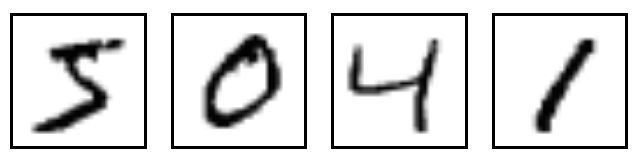
\includegraphics[width=0.75\textwidth]{images/5.png}
    \caption{MNIST 数据集示例图像, 每一副数字图像都是一个 $28 \times 28$ 的灰度图}
    \label{fig:mnist}
\end{figure}

\subsection{数据加载和预处理}

在处理MNIST数据集之前, 我们需要先加载数据. MNIST 数据集的官方网站提供了四个文件: 训练集图像 (\verb|train-images-idx3-ubyte|),
训练集标签 (\verb|train-labels-idx1-ubyte|), 测试集图像 (\verb|t10k-images-idx3-ubyte|)
和测试集标签 (\verb|t10k-labels-idx3-ubyte|).
这些文件都是特殊的二进制格式, 需要特殊的函数来读取. 在 C 语言中, 我们可以使用标准的文件 I/O 函数,
例如\verb|fopen|, \verb|fread| 和 \verb|fclose|, 来读取这些文件.

数据预处理是机器学习中的重要步骤, 它可以帮助我们改进模型的性能. 对于 MNIST 数据集, 一个常见的预处理步骤是归一化.
原始的 MNIST 图像是灰度图像, 像素值在 $0$ 到 $255$ 之间. 我们可以通过将像素值除以 $255$, 将它们归一化到 $0$ 到 $1$ 之间.
这样做可以使得模型的训练更加稳定, 因为所有的输入特征都在相同的尺度范围内.

% 在 MNIST 中, 每一张数字图片都是 $28 \times 28$ 像素的灰度位图. 每个像素值都是一个 $0 \sim 255$ 的整数. 为了后续计算,
% 我们统一为用 $0 \sim 1$ 的浮点数表示一个像素点的灰度.

这样每一副数字图片都转换成一个数字矩阵来表示
(原始项目由 Google Team 于 2015 年提供, 但目前已经下架, 这是网上找到的一个镜像 \cite{tensorflow2015mnist}):

\begin{figure}[htbp!]
    \centering
    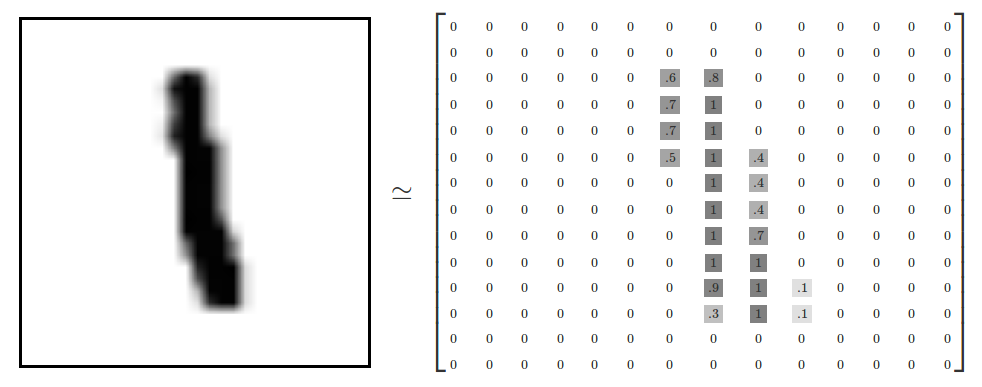
\includegraphics[width=0.95\textwidth]{images/MNIST-Matrix.png}
    \caption{MNIST 数据集的灰度表示, 每个像素位置用一个 $0 \sim 1$ 的浮点数表示黑色的深度,
        形成一个 $28 \times 28$ 的矩阵.}
    \label{fig:mnist_mateix}
\end{figure}

归一化过程可以用如下代码表示:
% 归一化:

\begin{verbatim}  
for(int i = 0; i < num_images; i++) {  
    for(int j = 0; j < image_size; j++) {  
        images[i][j] /= 255.0;  
    }  
}  
\end{verbatim}  

在这段代码中, \verb|num_images| 是图像的数量, \verb|image_size| 是每个图像的大小 (对于 MNIST 数据集,
\verb|image_size| 是 $28 \times 28 = 784$), \verb|images| 是一个二维数组, 存储了所有的图像数据.

\section{神经网络模型}
\label{sec::nn}

在本章中, 我们将详细介绍神经网络模型的基本概念和组成部分. 神经网络是一种模拟人脑神经元工作机制的计算模型,
由大量的神经元 (或称为节点) 按照一定的层次结构相互连接组成. 我们将首先描述神经网络的基本架构,
包括输入层、隐藏层和输出层, 以及这些层中的神经元如何通过权重和偏置进行连接. 接着, 我们将介绍神经网络的核心运算过程:
前向传播和反向传播, 这两个过程分别负责在网络中传递信息和调整网络参数. 最后, 我们将讨论神经网络的损失函数和优化方法,
这是神经网络学习从数据中学习和改进其性能的关键步骤.

\subsection{神经网络的架构}

神经网络模型主要由三种类型的层构成: 输入层、隐藏层和输出层\cite{goodfellow2016deep}.

{\bfseries 输入层}接收原始的数据输入, 例如图像、声音或文本. 这些数据通常需要经过预处理, 如归一化或向量化, 以便于网络处理.

{\bfseries 隐藏层}是神经网络的核心, 每个隐藏层都由多个神经元组成, 每个神经元都与上一层的所有神经元相连.
这些连接都有相应的权重, 代表了其在信息传递中的重要性. 隐藏层中的神经元会对输入数据进行一系列非线性变换, 从而提取出对于任务有用的特征\cite{lecun2015deep}.

隐藏层的计算通常涉及两个步骤: {\bfseries 线性变换}和 {\bfseries 非线性激活}. 对于第 $l$ 层的第 $i$ 个神经元,
其线性变换的结果 $y^{[l]}_i$ 可以用下面的公式表示:

\begin{equation}
    y^{[l]}_i = \sum_{j=1}^{n^{[l-1]}} w^{[l]}_{ij} x^{[l-1]}_j + b^{[l]}_i
\end{equation}

其中, $w^{[l]}_{ij}$ 是第 $l-1$ 层第 $j$ 个神经元到第 $l$ 层第 $i$ 个神经元的 {\bfseries 权重},
$x^{[l-1]}_j$ 是第 $l-1$ 层第 $j$ 个神经元的 {\bfseries 激活值} (是 $l - 1$ 层输出),
$b^{[l]}_i$ 是第 $l$ 层第 $i$ 个神经元的 {\bfseries 偏置项},
$n^{[l-1]}$ 是第 $l-1$ 层的神经元数量. 这个公式基本上是在计算第 $l$ 层第 $i$ 个神经元的输入,
也就是所有来自上一层的神经元的激活值与对应权重的乘积之和, 再加上偏置项.

然后, 这个线性变换的结果会被送入一个非线性激活函数 $g^{[l]}(\cdot)$, 得到第 $l$ 层第 $i$ 个神经元的激活值 $x^{[l]}_i$:

\begin{equation}
    x^{[l]}_i = g^{[l]}(y^{[l]}_i)
\end{equation}

其中, $g^{[l]}(\cdot)$ 是第 $l$ 层的激活函数, 可以是 sigmoid、tanh、ReLU 等函数. 这个公式的作用是将神经元的输入转化为输出,
加入非线性因素, 使得神经网络能够学习并表示更复杂的模式.

如果将上述两个公式结合起来, 可以得到从第 $l - 1$ 层第 $i$ 个神经元 $x^{[l - 1]}_i$
到第 $l$ 层第 $i$ 个的激活值 $x^{[l]}_i$ 的完整迭代计算公式:

\begin{equation}
    x^{[l]}_i = g^{[l]}\left(\sum_{j=1}^{n^{[l-1]}} w^{[l]}_{ij} x^{[l-1]}_j + b^{[l]}_i\right)
\end{equation}

从系统输入根据这个公式计算直到到最终输出的过程, 被称为神经网络的{\bfseries 前向传播}.

{\bfseries 输出层}将隐藏层的处理结果转化为我们想要的形式, 例如在分类问题中, 输出层会给出每个类别的预测概率.

此外, 每个神经元还有一个偏置项, 用于控制神经元的激活阈值的期望. 而每个神经元的输出激活函数, 
如 ReLU 或 sigmoid, 它们的目的除了增加模型的非线性表达能力\cite{glorot2011deep}, 
还根据需要归一化输出. 

其中 sigmoid 函数是神经网络中常用的一种激活函数, 其数学公式如下:

\begin{equation}
    \sigma(x) = \frac{1}{1 + e^{-x}}
\end{equation}
其中, $x$ 是输入, $e$ 是自然对数的底数. sigmoid函数的输出在 $0$ 和 $1$ 之间, 它能够将任意实数映射到 $(0, 1)$ 区间内,
因此常被用于输出层的激活函数, 表示分类问题的概率输出.

\subsection{反向传播}

% {\bfseries 前向传播}是神经网络计算输出的过程, 也就是将输入数据通过网络的每一层进行一系列的线性变换和非线性激活, 
% 最后得到输出结果\cite{goodfellow2016deep}. 对于每一层, 其计算过程可以用以下的公式表示:

% \begin{equation}  
% z^{[l]} = W^{[l]}a^{[l-1]} + b^{[l]}, a^{[l]} = g^{[l]}(z^{[l]})  
% \end{equation}   
% 其中, $W^{[l]}$ 和 $b^{[l]}$ 分别是第 $l$ 层的权重和偏置, $a^{[l-1]}$ 是上一层的激活值, $g^{[l]}(\cdot)$ 是激活函数.

对应前向传播, {\bfseries 反向传播}是神经网络学习 (即调整) 参数的过程, 也就是根据网络输出和真实目标之间的误差,
通过梯度下降等数值模型方法反向调整网络参数, 使得误差逐渐减小\cite{rumelhart1986learning}. 反向传播的计算过程可以用以下的公式表示:

\begin{eqnarray}
    \frac{\partial \mathcal{L}}{\partial x^{[l]}} &=& \frac{\partial \mathcal{L}}{\partial x^{[l]}} \cdot g'^{[l]}(x^{[l]}) \\
    \frac{\partial \mathcal{L}}{\partial W^{[l]}} &=& \frac{\partial \mathcal{L}}{\partial x^{[l]}} \cdot (x^{[l-1]})^T \\
    \frac{\partial \mathcal{L}}{\partial b^{[l]}} &=& \frac{\partial \mathcal{L}}{\partial x^{[l]}} \\
\end{eqnarray}
其中, $\mathcal{L}$ 是损失函数, $g'^{[l]}(\cdot)$ 是激活函数的导数.

最后, 我们使用梯度下降方法更新参数, 对于权重 $W$ 和偏置 $b$, 更新公式如下:

\begin{eqnarray}
    W^{[l]} &=& W^{[l]} - \alpha \frac{\partial \mathcal{L}}{\partial W^{[l]}} \\
    b^{[l]} &=& b^{[l]} - \alpha \frac{\partial \mathcal{L}}{\partial b^{[l]}}
\end{eqnarray}
这里, $\alpha$ 是 {\bfseries 学习率}, 一个超参数, 决定了参数更新的步长.

通过这样的方式, 网络的参数会逐渐调整, 使得预测误差逐渐减小.

\subsection{具体的 MNIST 神经网络的搭建和损失函数}

在针对 MNIST 的网络搭建中, 首先我们可以将每一个图片对应的矩阵看成 $28 \times 28 = 784$ 个数字组成的一维向量.
也就是我们这里实际上忽视了 2D 结构带来的信息, 这个会导致模型质量下降, 但是作为一个入门测试, 可以简化细节.
于是, 全部 MNIST 图片就是一堆位于 $784$ 维向量空间的点, 它构成了整个模型输入序列.

我们使用 softmax 函数最为非线性激活函数, 并且我们的最简单的神经网络只有一层中间层,
只有一个输入层和一个输出层, 没有隐藏层. 每个输入图像都被展平为一个一维数组, 并直接用于计算输出层的激活值.
这种神经网络也被称为{\bfseries 感知器} (Perceptron). 整个网络可以简化成一个函数:
\begin{equation}
    y = \mbox{softmax}(z) = \mbox{softmax}(W x + b).
\end{equation}
这里 $W$ 和 $b$ 分别代表权重矩阵和置偏向量, 在这个具体问题中, $W$ 是一个 $10 \times 784$ 的矩阵, 而 $b$ 是一个 $10$ 维的向量.
此外, 激活函数
\begin{equation}
    \mbox{softmax}(y_i) = \frac{e^{z_i}}{\sum_{j = 0}^{9}e^{z_j}},
\end{equation}
因此, 输出向量 $y$ 的每一个分量都是一个 $0 \sim 1$ 的浮点数, 它们的和是 $1$, 代表了一个具体的图片, 分别是 $0 \sim 9$ 的概率.
为了后续表示方便, 我们记线性运算结果为 $z = W x + b$, 它也是一个 $10$ 维的向量.

到此我们已经完成了前向传播的设计, 也就是输入一个具体的数字图片, 得到它是 $0 \sim 9$ 的概率. 接下来为了考虑向后传播, 我们需要设计损失函数,
也就是误差.

一个推荐的损失函数称为 ``交叉熵'' (cross-entropy)\cite{cover2006elements}. 这是一个来自信息论的概念, 定义如下:
$$
    H_{y'}(y) = -\sum_i y_i'\log(y_i)
$$
这里 $y$ 是计算所的关于 $i$ 的概率分布 (暂时大家可以理解为每个 $i$ 的可能性), 而 $y'$ 是实际的概率分布 (one-hot, 即只有一个确定的 $i$ 是 $1$, 其他是 $0$).
(仔细想想这个函数的意义) 某种意义上说, cross-entropy 度量了两个分布之间的区别. 在深度学习中, 交叉熵通常用作损失函数, 尤其是在处理分类问题时.

\section{神经网络的 C 语言实现}
\label{sec::implementation}

在这一部分, 我们将详细介绍如何在 C 语言中实现针对 MNIST 的具体神经网络. 我们将基于 Andrew Carter 的开源项目\cite{andrewcarteruk2018mnist}.

\subsection{MNIST 数据集的处理}

在 C 语言中, 我们可以使用结构体来表示 MNIST 数据集. 以下是在 C 语言中表示 MNIST 图像的结构体定义:

这段代码定义了一个结构体, 用于表示 MNIST 标签文件的头部.
\begin{verbatim}
    typedef struct mnist_label_file_header_t_ {  
        uint32_t magic_number;  
        uint32_t number_of_labels;  
    } __attribute__((packed)) mnist_label_file_header_t;          
\end{verbatim}

这段代码定义了一个结构体, 用于表示 MNIST 图像文件的头部.
\begin{verbatim}
    typedef struct mnist_image_file_header_t_ {  
    uint32_t magic_number;  
    uint32_t number_of_images;  
    uint32_t number_of_rows;  
    uint32_t number_of_columns;  
} __attribute__((packed)) mnist_image_file_header_t;  
\end{verbatim}

这段代码定义了一个结构体, 用于表示一个 MNIST 图像. 注意从这里的 \verb|pixels| 的类型可以看到,
数据库中表达像素的是一个短整数 ($8$ 个字长度), 范围是 $0 \sim 255$.
\begin{verbatim}
    typedef struct mnist_image_t_ {  
    uint8_t pixels[MNIST_IMAGE_SIZE];  
} __attribute__((packed)) mnist_image_t;  
\end{verbatim}

这段代码定义了一个结构体, 用于表示一个 MNIST 数据集, 包括图像、标签和数据集的大小.
\begin{verbatim}
    typedef struct mnist_dataset_t_ {  
    mnist_image_t * images;  
    uint8_t * labels;  
    uint32_t size;  
} mnist_dataset_t;  
\end{verbatim}

然后我们需要一些函数来处理这些数据:

\begin{verbatim}
    mnist_dataset_t * mnist_get_dataset(const char * image_path, 
                                        const char * label_path);  
    void mnist_free_dataset(mnist_dataset_t * dataset);  
    int mnist_batch(mnist_dataset_t * dataset, 
                    mnist_dataset_t * batch, 
                    int batch_size, 
                    int batch_number);  
\end{verbatim}

它们分别负责获取 MNIST 数据集, 释放 MNIST 数据集, 以及获取一个批次的数据.

有了这些数据结构和函数, 我们现在可以方便地加载和处理 MNIST 数据集了.

\subsection{神经网络的表示}

在 C 语言中, 我们使用结构体来表示神经网络的结构. 神经网络的主要组成部分包括偏置向量和权重矩阵. 以下是在 C 语言中表示神经网络的结构体定义:

\begin{verbatim}  
typedef struct neural_network_t_ {  
    float b[MNIST_LABELS];  
    float W[MNIST_LABELS][MNIST_IMAGE_SIZE];  
} neural_network_t;  
\end{verbatim}

在这个结构体中, \verb|b| 是一个数组, 存储了偏置向量, \verb|W| 是一个二维数组, 存储了权重矩阵.

同时, 我们也需要一个结构体来表示对应的梯度:

\begin{verbatim}  
typedef struct neural_network_gradient_t_ {  
    float b_grad[MNIST_LABELS];  
    float W_grad[MNIST_LABELS][MNIST_IMAGE_SIZE];  
} neural_network_gradient_t;  
\end{verbatim}

在这个结构体中, \verb|b_grad| 是一个数组, 存储了偏置向量的梯度, \verb|W_grad| 是一个二维数组, 存储了权重矩阵的梯度.

注意, 为了方便, 我们使用了固定大小的数组来存储偏置和权重, 以及它们的梯度. 这是因为在这个实现中, 我们只处理 MNIST 数据集, 所以可以预先知道数组的大小.

% \subsection{前向传播和反向传播的C语言实现}  

% 神经网络的训练过程主要包括前向传播和反向传播两个步骤. 在 C 语言中, 我们可以用一系列函数来实现这些步骤.

% \subsubsection{前向传播}  

前向传播的过程是通过输入数据和当前的权重和偏置, 计算神经网络的输出. 在 C 语言中, 我们可以使用 \verb|neural_network_hypothesis| 函数来实现这个过程:

\begin{verbatim}  
void neural_network_hypothesis(
    mnist_image_t * image, 
    neural_network_t * network, 
    float activations[MNIST_LABELS])  
{  
    int i, j;  
  
    for (i = 0; i < MNIST_LABELS; i++) {  
        activations[i] = network->b[i];  
  
        for (j = 0; j < MNIST_IMAGE_SIZE; j++) {  
            activations[i] 
            += network->W[i][j] 
                * PIXEL_SCALE(image->pixels[j]);  
        }  
    }  
  
    neural_network_softmax(activations, MNIST_LABELS);  
}  
\end{verbatim}

在这个函数中, 我们首先计算每个神经元的线性输出, 然后通过 softmax 函数将激活值转换为概率. 这里我们可以关注一下 softmax 的实现代码:

\begin{verbatim}
 void neural_network_softmax(float * activations, int length)
{
    int i;
    float sum, max;

    for (i = 1, max = activations[0]; i < length; i++) {
        if (activations[i] > max) {
            max = activations[i];
        }
    }

    for (i = 0, sum = 0; i < length; i++) {
        activations[i] = exp(activations[i] - max);
        sum += activations[i];
    }

    for (i = 0; i < length; i++) {
        activations[i] /= sum;
    }
}
\end{verbatim}

这段代码中的 softmax 函数采用了一种更为数值稳定的算法, 通过正则化激活值来防止指数运算的结果过大. 下面是这个函数的步骤:
\begin{enumerate}
    \item 找出激活值数组中的最大值. 这个步骤是为了提高数值稳定性, 防止在接下来的指数运算中出现过大的结果.
    \item 对每个激活值, 减去最大值, 然后计算指数. 这样做可以确保指数运算的结果不会过大. 同时, 计算所有指数值的和.
    \item 对每个指数值, 除以所有指数值的和. 这样做可以使得所有的输出值之和为 $1$, 满足概率分布的要求.
\end{enumerate}
这个函数的输入是一个浮点数数组和数组的长度, 输出是一个概率分布, 保存在原数组中.

\subsubsection{反向传播}

反向传播的过程是通过输出的误差, 反向计算每个权重和偏置的梯度. 在 C 语言中, 我们可以使用 \verb|neural_network_gradient_update| 函数来实现这个过程:

\begin{verbatim}  
float neural_network_gradient_update(
    mnist_image_t * image, 
    neural_network_t * network, 
    neural_network_gradient_t * gradient, 
    uint8_t label)  
{  
    float activations[MNIST_LABELS];  
    float b_grad, W_grad;  
    int i, j;  
  
    neural_network_hypothesis(image, network, activations);  
  
    for (i = 0; i < MNIST_LABELS; i++) {  
        // This is the gradient for a softmax bias input  
        b_grad 
        = (i == label) ? activations[i] - 1 : activations[i];  
  
        for (j = 0; j < MNIST_IMAGE_SIZE; j++) {  
            // The gradient for the neuron weight 
            // is the bias multiplied by the input weight  
            W_grad = b_grad * PIXEL_SCALE(image->pixels[j]);  
  
            // Update the weight gradient  
            gradient->W_grad[i][j] += W_grad;  
        }  
  
        // Update the bias gradient  
        gradient->b_grad[i] += b_grad;  
    }  
  
    // Cross entropy loss  
    return 0.0f - log(activations[label]);  
}  
\end{verbatim}

在这个函数中, 我们首先进行一次前向传播, 然后计算每个权重和偏置的梯度, 最后计算交叉熵损失.

这里注意梯度的计算, 比如对于每个标签 (即输出层的每个神经元), 计算偏置的梯度. 如果当前标签等于真实标签, 那么梯度就是激活值减 $1$,
否则就是激活值.

这是基于交叉熵损失函数和 softmax 激活函数的梯度计算.

在神经网络中, 激活值 $y$ 和偏置 $b$ 之间的关系通常通过以下公式表示:

$$
    y = \sigma(Wx + b)
$$

其中,
\begin{itemize}
    \item $y$ 是神经元的输出, 也就是激活值,
    \item $\sigma$ 是激活函数, 即 softmax 函数,
    \item $W$ 是神经元的权重,
    \item $x$ 是神经元的输入,
    \item $b$ 是神经元的偏置.
\end{itemize}

假设我们的网络输出经过 softmax 函数后为
$$
    \mathbf{y} = [y_1, y_2, \ldots, y_k],
$$
并且真实的标签为
$$
    \mathbf{t} = [t_1, t_2, \ldots, t_k],
$$
其中 $t_i$ 是一个 one-hot 编码, 即如果第 $i$ 个类别是正确的类别, $t_i = 1$, 否则 $t_i = 0$.

(离散) 交叉熵损失函数定义为:

$$
    L(\mathbf{y}, \mathbf{t}) = - \sum_{i=1}^{k} t_i \log y_i
$$

对于softmax函数,其定义为:

$$
    y_i = \frac{e^{z_i}}{\sum_{j=1}^{k} e^{z_j}}
$$

其中$\mathbf{z} = [z_1, z_2, \ldots, z_k]$是网络的原始输出.

当我们对交叉熵损失函数求关于$z_i$的偏导时,会发现一个非常好的性质:如果我们将交叉熵损失函数和softmax函数结合起来,其梯度形式非常简单:

$$
    \frac{\partial L}{\partial z_i} = y_i - t_i.
$$

事实上, 我们想要计算的是损失函数关于 $b$ 的偏导数 $\frac{\partial L}{\partial b_i}$.

由于 $y_i$ 是 $b_i$ 的函数, 我们可以使用链式法则:

$$
    \frac{\partial L}{\partial b_i} = \frac{\partial L}{\partial y_i} \frac{\partial y_i}{\partial b_i}
$$

对于交叉熵损失函数, 我们有:

$$
    \frac{\partial L}{\partial y_i} = - \frac{t_i}{y_i}
$$

对于 softmax 函数, 我们有:

$$
    \frac{\partial y_i}{\partial b_i} = y_i (1 - y_i) \quad \text{for} \quad i = j
$$

$$
    \frac{\partial y_i}{\partial b_j} = - y_i y_j \quad \text{for} \quad i \neq j
$$

当我们将这些放入到链式法则中, 我们可以得到:

$$
    \frac{\partial L}{\partial b_i} = \sum_{j=1}^{k} \frac{\partial L}{\partial y_j} \frac{\partial y_j}{\partial b_i}
$$

将 $j = i$ 和 $j \neq i$ 的情况分开,我们得到:

$$
    \frac{\partial L}{\partial b_i} = - t_i (1 - y_i) + \sum_{j \neq i} \frac{t_j}{y_j} (- y_j y_i) = y_i - t_i
$$

这就是我们最终的结果.

这就解释了为什么当标签等于真实标签时, 梯度是激活值减 $1$ ($y_i - 1$), 否则就是激活值 ($y_i - 0$).
这是由于在 one-hot 编码中, $t_i$ 只有一个元素是 $1$, 其余元素都是 $0$.

对于每个权重 $W_{ij}$, 它的梯度计算公式是:

$$
    \frac{\partial L}{\partial W_{ij}} = \frac{\partial L}{\partial z_i} \frac{\partial z_i}{\partial W_{ij}}
$$

在这里, $\frac{\partial L}{\partial z_i}$ 恰好就是前面计算的偏置梯度 $b_{\text{grad}}$,
$\frac{\partial z_i}{\partial W_{ij}}$ 是输入像素的值, 因为
$$
    z_i = W_{i1}x_1 + W_{i2}x_2 + \cdots + W_{ij}x_j + \cdots + b_i.
$$

所以, 权重的梯度就是偏置的梯度乘以输入的值:

$$
    W_{\text{grad}} = b_{\text{grad}} \times \text{PIXEL\_SCALE}(x_j)
$$

其中, \verb|PIXEL_SCALE| 是一个函数, 用来将像素值从原始的范围 (例如, $0$ 到 $255$) 转换到神经网络的输入范围 (例如, $0$ 到 $1$).

然后, 这个权重的梯度被用来更新 \verb|gradient->W_grad[i][j]|, 即该神经元对应的权重梯度:

\begin{verbatim}
    gradient->W_grad[i][j] += W_grad;    
\end{verbatim}

注意在这个 \verb|float neural_network_gradient_update| 函数中, 除了更新了梯度, 在返回值中还计算了交叉熵损失, 即当前误差.

\subsubsection{权重更新}

权重更新是神经网络训练过程中的一个重要步骤, 它是通过梯度下降算法来更新权重和偏置, 以便最小化损失函数.
在C语言中, 我们可以使用 \verb|neural_network_training_step| 函数来实现这个过程:

\begin{verbatim}  
float neural_network_training_step(
    mnist_dataset_t * dataset, 
    neural_network_t * network, 
    float learning_rate)  
{  
    neural_network_gradient_t gradient;  
    float total_loss;  
    int i, j;  
  
    // Zero initialise gradient for weights and bias vector  
    memset(&gradient, 0, sizeof(neural_network_gradient_t));  
  
    // Calculate the gradient and the loss 
    // by looping through the training set  
    for (i = 0, total_loss = 0; i < dataset->size; i++) {  
        total_loss 
        += neural_network_gradient_update(&dataset->images[i], 
                                          network, &gradient, 
                                          dataset->labels[i]);  
    }  
  
    // Apply gradient descent to the network  
    for (i = 0; i < MNIST_LABELS; i++) {  
        network->b[i] 
        -= learning_rate * gradient.b_grad[i] 
            / ((float) dataset->size);  
  
        for (j = 0; j < MNIST_IMAGE_SIZE; j++) {  
            network->W[i][j] 
            -= learning_rate * gradient.W_grad[i][j] 
                / ((float) dataset->size);  
        }  
    }  
  
    return total_loss;  
}  
\end{verbatim}

这段代码实现了神经网络的一个训练步骤, 具体步骤如下:
\begin{enumerate}
    \item 首先, 对权重和偏置的梯度进行零初始化.
    \item 然后, 通过遍历训练集中的所有样本, 调用
          \verb|neural_network_gradient_update| 函数来计算每个样本对梯度的贡献,
          并将这个贡献累加到之前的梯度上. 同时, 计算每个样本的损失, 并将这个损失累加到总损失上.
    \item 在计算完所有样本的梯度和损失后, 使用梯度下降法来更新神经网络的参数. 对于每个参数, 其更新的公式是:
          $$
              \theta = \theta - \alpha \frac{\partial L}{\partial \theta}
          $$
          其中, $\theta$ 是参数 (例如, 权重或偏置), $\alpha$ 是学习率,
          $\frac{\partial L}{\partial \theta}$ 是参数的梯度. 注意这里的梯度是所有样本的梯度的平均值, 这就是为什么我们要将梯度除以样本的数量.
    \item 最后, 返回总损失. 这可以用来监控训练过程.
\end{enumerate}

这个函数的输入是一个训练集、一个神经网络和一个学习率,输出是这个训练步骤的总损失.

这就是神经网络训练的基本过程. 在实际训练中, 我们通常会重复这个过程多个周期 (即, 遍历训练集多次), 直到损失收敛或者达到预设的最大训练周期.

\subsubsection{批量训练过程详解}

批量训练是神经网络训练过程中的一个重要步骤, 它是通过在一批数据上进行梯度下降来更新权重和偏置, 以便最小化损失函数.
以下是在 C 语言中进行批量训练的详细过程:

\begin{verbatim}  
#define STEPS 1000  
#define BATCH_SIZE 100  
  
int main(int argc, char *argv[])  
{  
    mnist_dataset_t * train_dataset, * test_dataset;  
    mnist_dataset_t batch;  
    neural_network_t network;  
    float loss, accuracy;  
    int i, batches;  
  
    // Read the datasets from the files  
    train_dataset 
    = mnist_get_dataset(train_images_file, 
                        train_labels_file);  
    test_dataset 
    = mnist_get_dataset(test_images_file, 
                        test_labels_file);  
\end{verbatim}

首先, 我们从文件中读取训练集和测试集. 这两个数据集分别用于训练神经网络和评估其性能.

\begin{verbatim}  
    // Initialise weights and biases with random values  
    neural_network_random_weights(&network);  
\end{verbatim}

然后, 我们使用随机值初始化神经网络的权重和偏置. 注意这个实现过程:

\begin{verbatim}
void neural_network_random_weights(neural_network_t * network) {  
    int i, j;  
  
    // Initialize the seed for random number generator  
    srand(time(NULL));  
  
    // Loop through each output neuron  
    for (i = 0; i < MNIST_LABELS; i++) {  
        // Randomly initialize the bias for each output neuron  
        network->b[i] = ((float) rand() / (RAND_MAX)) - 0.5;  
  
        // Loop through each input pixel  
        for (j = 0; j < MNIST_IMAGE_SIZE; j++) {  
            // Randomly initialize the weight for each input pixel  
            network->W[i][j] = ((float) rand() / (RAND_MAX)) - 0.5;  
        }  
    }  
}  
\end{verbatim}

在这个函数中:

\verb|srand(time(NULL))| 是用来初始化随机数生成器的种子, 这样每次运行程序时生成的随机数序列都会不同.

对于每个输出神经元, 我们随机初始化其偏置和权重并将其转换到 $[-0.5, 0.5]$ 的范围. 
这种随机初始化的方法可以保证神经网络的权重和偏置在开始训练时不会全部相同, 这对于神经网络的训练是很重要的. 
如果所有的权重和偏置都相同, 那么在反向传播过程中, 所有的神经元都会得到相同的更新, 这样神经网络就无法学习到有用的模式.

\begin{verbatim}  
    // Calculate how many batches 
    // (so we know when to wrap around)  
    batches = train_dataset->size / BATCH_SIZE;  
\end{verbatim}

接下来, 我们计算训练集可以被分成多少个批次. 这是因为在每一步训练中, 我们将在一个批次上进行梯度下降.
批次的大小是一个超参数, 可以根据具体的应用和计算资源进行调整.

\begin{verbatim}  
    for (i = 0; i < STEPS; i++) {  
        // Initialise a new batch  
        mnist_batch(train_dataset, 
                    &batch, 
                    100, 
                    i % batches);  
  
        // Run one step of gradient descent 
        // and calculate the loss  
        loss = neural_network_training_step(&batch, 
                                            &network, 
                                            0.5);  
\end{verbatim}

然后, 我们开始训练过程. 在每一步训练中, 我们首先初始化一个新的批次. 然后,
我们在这个批次上运行一步梯度下降, 并计算损失.

\begin{verbatim}  
        // Calculate the accuracy using the whole test dataset  
        accuracy = calculate_accuracy(test_dataset, 
                                      &network);  
  
        printf(
            "Step %04d\tAverage Loss: %.2f\tAccuracy: %.3f\n", 
            i, 
            loss / batch.size, 
            accuracy);  
    }  
\end{verbatim}

在每一步训练之后, 我们使用整个测试集来计算精度. 这可以帮助我们监控神经网络的训练过程, 并调整超参数以优化性能.
这里注意一下准确率的估计:

\begin{verbatim}
/**  
 * 计算神经网络在数据集上的预测准确率。  
 */  
float calculate_accuracy(mnist_dataset_t * dataset, 
                         neural_network_t * network)  
{  
    float activations[MNIST_LABELS], max_activation;  
    int i, j, correct, predict;  
  
    // 遍历整个数据集  
    for (i = 0, correct = 0; i < dataset->size; i++) {  
        // 使用神经网络计算每个图像的激活值  
        neural_network_hypothesis(&dataset->images[i], 
                                  network, 
                                  activations);  
  
        // 设置predict为激活值最大的索引  
        for (j = 0, predict = 0, max_activation = activations[0]; 
             j < MNIST_LABELS; 
             j++) {  
            if (max_activation < activations[j]) {  
                max_activation = activations[j];  
                predict = j;  
            }  
        }  
  
        // 如果我们预测的标签正确,就增加正确计数  
        if (predict == dataset->labels[i]) {  
            correct++;  
        }  
    }  
  
    // 返回我们预测正确的百分比作为准确率  
    return ((float) correct) / ((float) dataset->size);  
}  
\end{verbatim}

最后, 我们清理训练集和测试集, 释放它们占用的内存.
\begin{verbatim}  
    // Cleanup  
    mnist_free_dataset(train_dataset);  
    mnist_free_dataset(test_dataset);  
  
    return 0;  
}  
\end{verbatim}

\section{模型训练和评估}
\label{sec::training}

\subsection{模型训练的过程}

模型训练的过程是一个迭代的过程, 其中我们反复更新模型的参数以最小化损失函数. 在每一步训练中,
我们首先选择一个数据批次, 然后计算该批次数据上的损失和梯度, 最后使用梯度下降算法来更新模型的参数.

模型训练的过程中有几个重要的超参数需要选择, 包括学习率, 批次大小, 和训练步骤. 学习率决定了我们在每一步中更新参数的幅度,
批次大小决定了我们在每一步中使用的数据量, 而训练步骤则决定了我们进行多少步的训练.

\subsection{计算和展示训练过程中的损失}

在训练过程中, 我们需要计算和展示损失以监控训练的进展. 我们可以在每一步训练后计算当前批次数据上的平均损失,
然后将这个损失添加到一个列表中. 这样, 我们就可以绘制一个损失随时间的曲线, 以便我们可以看到损失是否随着时间的推移而减少, 以及是否存在过拟合或欠拟合的问题.

\subsection{使用测试数据集评估模型的性能}

在模型训练完成后, 我们需要使用测试数据集来评估模型的性能. 这是因为我们想知道模型在未见过的数据上的性能,
而不仅仅是训练数据. 我们可以计算模型在测试数据集上的损失和精度, 以得到模型的性能指标.

\section{结果和讨论}
\label{sec::results}

\begin{figure}[htbp!]
    \centering
    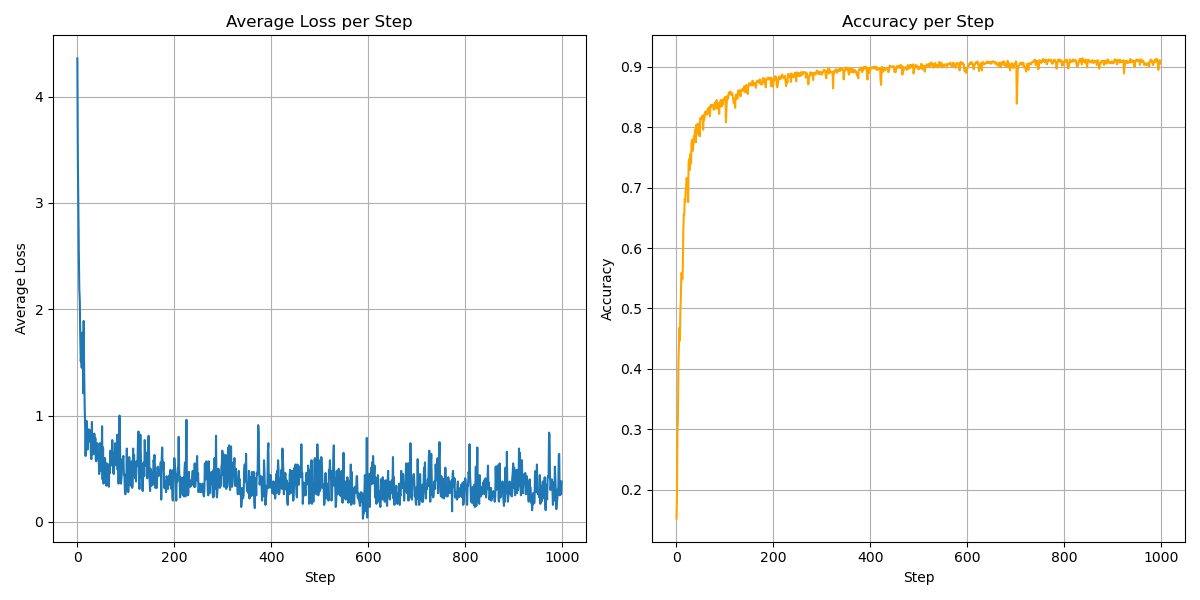
\includegraphics[width=0.95\textwidth]{images/result.png}
    \caption{MNIST 数据测试结果. 左: 损失函数随步长变化曲线; 右: 准确率随步长变化曲线.}
    \label{fig::result}
\end{figure}

根据实际的计算结果, 我们可以看到模型的平均损失 (Average Loss) 随着训练步骤的增加而逐渐减小,
而准确率 (Accuracy) 则逐渐增加. 这表明模型在训练过程中逐渐学习并改进了其预测能力.

\begin{itemize}
    \item 初始阶段 (Step 0000-0005): 模型的平均损失较高, 准确率较低, 这表明模型刚开始学习, 尚未很好地适应数据集.
    \item 中间阶段 (Step 0006-0040): 随着训练的进行, 平均损失显著下降, 准确率显著提升, 显示出模型性能的快速改进.
    \item 稳定阶段 (Step 0041-0180): 在这个阶段, 平均损失继续缓慢下降, 而准确率趋于稳定, 表明模型已经接近其性能极限.
\end{itemize}

这里影响模型性能的因素分析可能有:
\begin{enumerate}
    \item {\bfseries 模型架构}: 模型的层数、神经元数量、激活函数等都会影响其学习能力和性能.
    \item {\bfseries 训练数据}: MNIST 数据集的质量、多样性和代表性对模型性能有直接影响.
    \item {\bfseries 训练过程}: 包括学习率、优化算法、正则化技术、早停法 (early stopping) 等都会影响训练效果.
    \item {\bfseries 超参数设置}: 如批量大小 (batch size)、迭代次数 (epochs) 等, 需要仔细调整以获得最佳性能.
    \item {\bfseries 随机性}: 由于初始化权重的随机性, 每次训练的结果可能略有不同.
\end{enumerate}

而对应可能的改进方法有:
\begin{enumerate}
    \item 调整模型架构: 可以尝试增加网络深度 (如使用更深的卷积神经网络) 或宽度 (增加卷积层的过滤器数量) 来提高模型的学习能力.
    \item 数据增强: 通过对训练数据进行旋转、缩放、裁剪等操作, 可以提高模型的泛化能力.
    \item 超参数调优: 使用如网格搜索、随机搜索或贝叶斯优化等方法来找到最佳的超参数组合.
    \item 正则化技术: 应用如 dropout、L1/L2 正则化等技术来防止过拟合.
    \item 学习率调度: 使用学习率衰减或预热等策略, 以优化训练过程.
    \item 集成方法: 使用模型集成技术, 如 bagging 或 boosting, 来提高整体性能.
    \item 探索不同的优化算法: 如 Adam、RMSprop 等, 可能会对模型性能产生影响.
\end{enumerate}

实际计算表明, 模型在 MNIST 数据集上的表现随着训练的进行而稳步提升. 然而, 为了进一步提升模型的性能,
需要对模型架构、训练过程和超参数进行细致的调整和优化. 此外, 考虑到模型在训练后期准确率趋于稳定, 可能已经接近其性能瓶颈,
进一步的改进可能需要更复杂的模型或更高级的技术.

\section{总结和展望}
\label{sec::conclusion}

在本文中, 我们详细介绍了如何使用 C 语言实现神经网络, 并对模型的训练和评估过程进行了详细的描述.
我们讨论了如何选择超参数, 如何计算和展示训练过程中的损失, 以及如何使用测试数据集评估模型的性能.
我们还提供了一个 Python 程序来根据训练结果绘制损失和精度随时间变化的曲线图.

然而, 本文中的实现还有很多可以改进和扩展的地方. 例如, 我们可以尝试使用不同的优化算法,
如 Adam 或 RMSProp, 来提高模型的训练效率. 我们也可以尝试添加更多的隐藏层或使用不同的激活函数, 来增加模型的复杂性和表达能力.
此外, 我们还可以尝试使用不同的数据集, 如 CIFAR-10 或 ImageNet, 来测试模型的性能.

总的来说, 虽然神经网络和深度学习是一个复杂的领域, 但通过理解和实现模型的基本组件,
我们可以更好地理解这些模型是如何工作的, 以及如何改进和优化这些模型.
在未来, 我们希望能进一步探索这个领域, 提供更多的实用工具和资源, 以帮助读者更好地理解和应用神经网络和深度学习.

\subsection{进一步的思考}

首先我们应该思考, 我们在数学上实际求解了一个怎样的优化问题. 而理论上的最优解应该在哪里?

粗略地看, 这似乎是一个简单的最小二乘问题: 已知 $x^{[0]}$ 为 $60000$ 个手写图片, 
求 $W$ 和 $b$, 使分类器
$$
x^{[1]}_i = g\left(\sum_{j = 1}^{784} w_{ij} x^{[0]}_j + b_i\right)
$$
在损失函数 entropy-cross 下误差最小. 注意这里 $g$ 是 softmax 函数, 我们的网络本质上只有一层,
即 $l = 1$.

上面这个最小二乘问题显然有唯一解 $W^*, b^*$, 但这个是我们追求的解么?

回答显然是否定的. 因为最小二乘解 $W^*, b^*$ 和输入数据 $x^{[0]}, y'$ 是绑定的 (这里 $y'$ 是标签, 
也就是真解). 它的 ``最优性'' 只体现在这 $60000$ 个数据中. 哪怕再增加或减少一对数据, 都会影响这个解.

而我们追求的, 是用这 $60000$ 个数据, 获得对 {\bfseries 全部可能的手写数字} 的最佳识别参数 $W$ 和 $b$.
显然, 我们的目标集合是一个无穷集 (概念上是无穷的, 但实际上仍然是有限集. 
也就是整个人类文明中出现的全部的最广义上的手写的阿拉伯数字. 最广义, 比如挖掘机写的也算. )

那么这种最优性如何体现? 回答是做不到最优. 因为我们无法保证我们已有 $60000$ 个数据的充分代表性.
我们只能说, 如果我们收集的这 $60000$ 个数据. 已经在统计意义上充分代表了全体手写数字, 
那么我们可以根据这 $60000$ 个数据提供的信息, 获得手写数字的特征. 

从这个角度说, 我们追求的, 和实际获得的, 都是一种统计学意义上的 ``最优''. 增加一个或若干个数据,
不会对我们的结果造成重大影响. 除非新增的数据, 在统计意义上多到影响我们整个数据集的特征. 也就是说,
我们其实是在做统计, 我们获得的, 其实是统计意义上的各种特征. 我们的问题和网络虽然简单, 但这个基本点,
和更加复杂的网络是一致的.

最后我们用一个有趣的观察结束我们的讨论: 在我们的问题中, 这些特征是可视的.

\begin{figure}
    \centering
    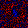
\includegraphics[width=0.18\textwidth]{images/weight-0.png}
    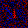
\includegraphics[width=0.18\textwidth]{images/weight-1.png}
    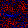
\includegraphics[width=0.18\textwidth]{images/weight-2.png}
    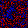
\includegraphics[width=0.18\textwidth]{images/weight-3.png}
    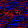
\includegraphics[width=0.18\textwidth]{images/weight-4.png}
    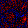
\includegraphics[width=0.18\textwidth]{images/weight-5.png}
    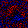
\includegraphics[width=0.18\textwidth]{images/weight-6.png}
    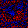
\includegraphics[width=0.18\textwidth]{images/weight-7.png}
    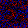
\includegraphics[width=0.18\textwidth]{images/weight-8.png}
    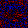
\includegraphics[width=0.18\textwidth]{images/weight-9.png}
    \caption{神经网络的权重可视化. 从左到右, 从上到下, 依次为 $0 \sim 9$ 的权重. 
    红色表示匹配度高的像素点, 蓝色表示匹配度低的像素点.}
\end{figure}

在这些权重中, 我们用颜色表示权重的大小. 红色表示权重较大, 蓝色表示权重较小. 我们可以看到,
这实际上体现了我们的网络是如何 ``看'' 手写数字的. 也就是说, 我们的网络实际上是在学习,
如何从这些像素点中, 提取出手写数字的特征. 这些特征, 实际上是我们的网络学习到的 ``知识''.

最后, 我们再讨论一下, 是否可以用区区 $60000$ 个手写数字样本, 获得更加好的识别效果. 或者说, 
更接近我们之前讨论的广义的最优解. 似乎从直觉上, 这是不可能的. 但是, 
这么想本身就陷入了一个思维误区, 就是这个最优解难道是存在且唯一的么? 显然, 
我们真正应该否定掉的是获得一个  ``存在且唯一'' 的最优解. 而这个命题, 从提出时就是不成立的.
我们真正需要的是一种对手写字体特征分布的描述, 也就是哪些像素点更可能出现在哪些数字上. 
从这个意义上说, 我们应该充分利用统计学知识, 去还原这个分布的信息. 从这个意义上说, 
$60000$ 的样本并不是少数了. 这里顺便指出我们的模型的一个缺陷, 就是我们没有去统计像素之间的关系.
也就是说, 在判定某个数字时, 如果某个像素是深红色, 那么它周围的像素更有可能是红色还是蓝色? 再远一点呢?
这个统计, 本质上在还原数字的二维结构. 但注意我们的模型的第一步, 就把二位数组拉成了一维, 
从而丢失了大部分二维信息. 实际上, 更好的设计, 可以让这 $60000$ 张图片训练出的网络, 
在后续的测试中获得 $99\%$ 以上的正确率, 从而成为一个实际可用的手写数字识别器. 
不过这个已经超过了我们目前的讨论范围.

\bibliographystyle{plain}
\bibliography{references}


\end{document}